\documentclass{beamer}[10]
\usepackage{pgf}
\usepackage{beamerthemesplit}
\usepackage{array}
\usepackage{wrapfig}
\usepackage{varwidth}
%\usepackage{enumitem}
\usepackage{listings}
\lstset{language=bash,
	basicstyle=\ttfamily\scriptsize,		
	keywordstyle=\color{blue}\ttfamily,
	morekeywords={peter@kbpet},
	alsoletter={:~$},
	morekeywords=[2]{peter@kbpet:},
	keywordstyle=[2]{\color{red}},
	literate={\$}{{\textcolor{red}{\$}}}1 
	{:}{{\textcolor{red}{:}}}1
	{~}{{\textcolor{red}{\textasciitilde}}}1,
	breaklines=true,
	numbers=none,
	numbersep=5pt,
	stepnumber=1
}
\usepackage{algorithm,algpseudocode}
\usepackage{hyperref}
%\usepackage{pdfpc-commands}
\usepackage{pgfpages}

\usepackage{tikz}
\usetikzlibrary{er,positioning}
\usepackage{float}
\usepackage{subcaption}
\usepackage{xcolor}
\usepackage[acronym]{glossaries}

%\usepackage{natbib}
\bibliographystyle{apalike}

\definecolor{kugreen}{RGB}{50,93,61}
\definecolor{kugreenlys}{RGB}{132,158,139}
\definecolor{kugreenlyslys}{RGB}{173,190,177}
\definecolor{kugreenlyslyslys}{RGB}{214,223,216}
\definecolor{kublue}{RGB}{0,101,163}
\definecolor{kubluelys}{RGB}{132,158,139}
\definecolor{kubluelyslys}{RGB}{173,190,177}
\definecolor{kubluelyslyslys}{RGB}{214,223,216}
\setbeamercovered{transparent}
\mode<presentation>
\usetheme[numbers,totalnumber,compress,sidebarshades]{PaloAlto}
%\setbeamertemplate{footline}[frame number]

\usecolortheme[named=kublue]{structure}
\useinnertheme{circles}
\usefonttheme[onlymath]{serif}
\setbeamercovered{transparent}
\setbeamertemplate{blocks}[rounded][shadow=true]
%\setbeameroption{show notes on second screen}
%\setbeameroption{show notes}

\logo{
\includegraphics[width=1.5cm]{gfx/eth_logo_kurz_pos}}
\title{Semester Project}
\subtitle{Map Fusion for Collaborative UAV SLAM}
\author{Andreas Ziegler}
\institute{V4RL \\ ETH Zürich}
\date{12th of January 2017}

\newcommand{\setlistspacing}[2]{\def\@ld{#1}\expandafter\def\csname
	@list\romannumeral\@ld \endcsname{\leftmargin\csname
		leftmargin\romannumeral\@ld \endcsname
		\topsep    #2
		\parsep    0\p@   \@plus\p@
		\itemsep   #2}}
\makeatother

\newacronym{KF}{KF}{key frame}

\begin{document}

\frame { \frametitle{Semester Project}
	\begin{center}
	\LARGE Semester Project \\
	- \\
	Map Fusion for Collaborative UAV SLAM\\
	- \\
	\includegraphics*[height=0.6cm]{gfx/eth_logo_kurz_pos.eps} \hfill
	\includegraphics*[height=0.6cm]{gfx/v4rl_logo} \hfill
	\includegraphics*[height=0.6cm]{gfx/asl_logo_right.pdf}
	\end{center}
}

\frame { \frametitle{Contents}
	\tableofcontents
}

\section{Introduction}
\frame{\tableofcontents[currentsection]}

\frame{ \frametitle{Introduction}
	\begin{itemize}
	\visible<1-5>{
	\item SLAM is one of the most important challenges for robots to be autonomous.
	}
	\visible<2-5>{
	\item For a team of UAVs collaboratively performing tasks, a common map is required
  }
	\visible<3-5>{
	\item To merge two maps, the alignment of them has to be found
	}
  \visible<4-5>{
  \item To build a common map from the maps of the UAVs, the maps need to be merged
  }
	\visible<5>{	
	\item Redundant information should be removed to achieve a better performance
	}
	\end{itemize}
}
\note[enumerate]
{
	\item for many interactive systems, especially for robotic systems interacting with humans.
	\item any such tracking approach has to balance plasticity versus drift, in particular when an object should be re-detected after loss of tracking.
}

\section{Motivation}
\frame{\tableofcontents[currentsection]}

\frame{ \frametitle{Motivation}
	\begin{itemize}
  \visible<1-4>{
\item Using multiple \gls{KF} matches to guarantee no false map merging
  }
  \visible<2-4>{
  \item Using multiple \gls{KF} matches to obtain an optimal map alignment
  }
  \visible<3-4>{
  \item Perform \gls{KF} culling to remove redundant information as bundle adjustment complexity grows with the number of \gls{KF}
  }
  \visible<4>{
  \item A multi agent SLAM system based on ORB-SLAM2 should be extended
  }
  \end{itemize}
  \visible<3>{\cite{Mur-Artal2015}}
  \visible<4>{\cite{Mur-Artal2015,Mur-Artal2016}}
}

\section{Map merging}
\frame{\tableofcontents[currentsection]}

\subsection{Old approach}
\frame{	\frametitle{Map merging - Old approach}
   Old approach:
	\begin{itemize}
    \item As soon as a \gls{KF} match was detected, maps were merged
	\end{itemize}
}

\subsection{New approach}
\frame{
  \frametitle{Map merging - New approach}
  New approach:
	\begin{enumerate}
    \pause
  \item After a \gls{KF} match is found skip $m$ \gls{KF} before processing the next \gls{KF} match
    \pause
  \item Wait for $n$ \gls{KF} matches
    \pause
  \item Merge the two maps with the transformation of one of the \gls{KF} matches
    \pause
  \item Fuse map points in the ($n-1$) \gls{KF} matches
    \pause
    \item Pose graph optimization over essential graph
    \pause
    \item Global bundle adjustment
	\end{enumerate}
}

\frame{
  \frametitle{Map merging - New approach}
  \only<1>{
  Find $n$ \gls{KF} matches
  \begin{center}
  \begin{tikzpicture}
    \coordinate (A1) at (0, 3);
    \coordinate (A1MP1) at (-0.5, 3.5);
    \coordinate (A1MP2) at (0, 3.75);
    \coordinate (A1MP3) at (0.5, 3.5);

    \coordinate (B1) at (4, 3);
    \coordinate (B1MP1) at (3.2, 3.15);
    \coordinate (B1MP2) at (3.4, 3.6);
    \coordinate (B1MP3) at (3.9, 3.5);

    \coordinate (C1) at (4, 6);
    \coordinate (C1MP1) at (3.5, 6.5);
    \coordinate (C1MP2) at (3.25, 6.0);
    \coordinate (C1MP3) at (3.5, 5.5);

    \coordinate (A2) at (0, 0);
    \coordinate (A2MP1) at (-0.5, 0.5);
    \coordinate (A2MP2) at (0, 0.75);
    \coordinate (A2MP3) at (0.5, 0.5);

    \coordinate (B2) at (8, 0);
    \coordinate (B2MP1) at (7.2, 0.15);
    \coordinate (B2MP2) at (7.4, 0.6);
    \coordinate (B2MP3) at (7.9, 0.5);

    \coordinate (C2) at (8, 6);
    \coordinate (C2MP1) at (7.5, 6.5);
    \coordinate (C2MP2) at (7.25, 6.0);
    \coordinate (C2MP3) at (7.5, 5.5);

    \node [fill=orange!70, circle,inner sep=2pt, text width=0.1mm] at (A1) {};
    \node [fill=green!70, circle,inner sep=2pt, text width=0.1mm] at (A1MP1) {};
    \node [fill=green!70, circle,inner sep=2pt, text width=0.1mm] at (A1MP2) {};
    \node [fill=green!70, circle,inner sep=2pt, text width=0.1mm] at (A1MP3) {};
    \draw [green!50, dashed, line width=0.05cm] (A1) to (A1MP1);
    \draw [green!50, dashed, line width=0.05cm] (A1) to (A1MP2);
    \draw [green!50, dashed, line width=0.05cm] (A1) to (A1MP3);

    \node [fill=orange!70, circle, inner sep=2pt, text width=0.1mm] at (B1) {};
    \node [fill=green!70, circle, inner sep=2pt, text width=0.1mm] at (B1MP1) {};
    \node [fill=green!70, circle, inner sep=2pt, text width=0.1mm] at (B1MP2) {};
    \node [fill=green!70, circle, inner sep=2pt, text width=0.1mm] at (B1MP3) {};
    \draw [green!50, dashed, line width=0.05cm] (B1) to (B1MP1);
    \draw [green!50, dashed, line width=0.05cm] (B1) to (B1MP2);
    \draw [green!50, dashed, line width=0.05cm] (B1) to (B1MP3);

    \node [fill=orange!70, circle,inner sep=2pt, text width=0.1mm] at (C1) {};
    \node [fill=green!70, circle, inner sep=2pt, text width=0.1mm] at (C1MP1) {};
    \node [fill=green!70, circle, inner sep=2pt, text width=0.1mm] at (C1MP2) {};
    \node [fill=green!70, circle, inner sep=2pt, text width=0.1mm] at (C1MP3) {};
    \draw [green!50, dashed, line width=0.05cm] (C1) to (C1MP1);
    \draw [green!50, dashed, line width=0.05cm] (C1) to (C1MP2);
    \draw [green!50, dashed, line width=0.05cm] (C1) to (C1MP3);

    \node [fill=blue!70, circle,inner sep=2pt, text width=0.1mm] at (A2) {};
    \node [fill=green!70, circle,inner sep=2pt, text width=0.1mm] at (A2MP1) {};
    \node [fill=green!70, circle,inner sep=2pt, text width=0.1mm] at (A2MP2) {};
    \node [fill=green!70, circle,inner sep=2pt, text width=0.1mm] at (A2MP3) {};
    \draw [green!50, dashed, line width=0.05cm] (A2) to (A2MP1);
    \draw [green!50, dashed, line width=0.05cm] (A2) to (A2MP2);
    \draw [green!50, dashed, line width=0.05cm] (A2) to (A2MP3);

    \node [fill=blue!70, circle,inner sep=2pt, text width=0.1mm] at (B2) {};
    \node [fill=green!70, circle,inner sep=2pt, text width=0.1mm] at (B2MP1) {};
    \node [fill=green!70, circle,inner sep=2pt, text width=0.1mm] at (B2MP2) {};
    \node [fill=green!70, circle,inner sep=2pt, text width=0.1mm] at (B2MP3) {};
    \draw [green!50, dashed, line width=0.05cm] (B2) to (B2MP1);
    \draw [green!50, dashed, line width=0.05cm] (B2) to (B2MP2);
    \draw [green!50, dashed, line width=0.05cm] (B2) to (B2MP3);

    \node [fill=blue!70, circle,inner sep=2pt, text width=0.1mm] at (C2) {};
    \node [fill=green!70, circle, inner sep=2pt, text width=0.1mm] at (C2MP1) {};
    \node [fill=green!70, circle, inner sep=2pt, text width=0.1mm] at (C2MP2) {};
    \node [fill=green!70, circle, inner sep=2pt, text width=0.1mm] at (C2MP3) {};
    \draw [green!50, dashed, line width=0.05cm] (C2) to (C2MP1);
    \draw [green!50, dashed, line width=0.05cm] (C2) to (C2MP2);
    \draw [green!50, dashed, line width=0.05cm] (C2) to (C2MP3);

    \draw [orange!50, line width=0.05cm] (A1) to (B1);
    \draw [orange!50, line width=0.05cm] (B1) to (C1);
    \draw [blue!50, line width=0.05cm] (A2) to (B2);
    \draw [blue!50, line width=0.05cm] (B2) to (C2);

    \draw [red!50, line width=0.05cm, dashed] (A1) to (A2);
    \draw [red!50, line width=0.05cm, dashed] (B1) to (B2);
    \draw [red!50, line width=0.05cm, dashed] (C1) to (C2);
  \end{tikzpicture}
  \end{center}
  }
  \only<2>{
  Merge the two maps and fuse map points
  \begin{center}
  \begin{tikzpicture}
    \coordinate (A1) at (0, 0.25);
    \coordinate (A1MP1) at (-0.5, 0.75);
    \coordinate (A1MP2) at (0, 1.0);
    \coordinate (A1MP3) at (0.5, 0.75);

    \coordinate (B1) at (4, 0.25);
    \coordinate (B1MP1) at (3.2, 0.15);
    \coordinate (B1MP2) at (3.4, 0.6);
    \coordinate (B1MP3) at (3.9, 0.5);

    \coordinate (C1) at (4, 5);
    \coordinate (C1MP1) at (3.5, 5.5);
    \coordinate (C1MP2) at (3.25, 5.0);
    \coordinate (C1MP3) at (3.5, 4.5);

    \coordinate (A2) at (0, 0);

    \coordinate (B2) at (5.5, 0);

    \coordinate (C12) at (4.5, 5.0);
    \coordinate (C2) at (5.5, 5);

    \node [fill=orange!70, circle,inner sep=2pt, text width=0.1mm] at (A1) {};
    \node [fill=green!30, circle,inner sep=2pt, text width=0.1mm] at (A1MP1) {};
    \node [fill=green!30, circle,inner sep=2pt, text width=0.1mm] at (A1MP2) {};
    \node [fill=green!30, circle,inner sep=2pt, text width=0.1mm] at (A1MP3) {};
    \draw [green!50, line width=0.05cm] (A1) to (A1MP1);
    \draw [green!50, line width=0.05cm] (A1) to (A1MP2);
    \draw [green!50, line width=0.05cm] (A1) to (A1MP3);

    \node [fill=orange!70, circle,inner sep=2pt, text width=0.1mm] at (B1) {};
    \node [fill=green!30, circle, inner sep=2pt, text width=0.1mm] at (B1MP1) {};
    \node [fill=green!30, circle, inner sep=2pt, text width=0.1mm] at (B1MP2) {};
    \node [fill=green!30, circle, inner sep=2pt, text width=0.1mm] at (B1MP3) {};
    \draw [green!50, line width=0.05cm] (B1) to (B1MP1);
    \draw [green!50, line width=0.05cm] (B1) to (B1MP2);
    \draw [green!50, line width=0.05cm] (B1) to (B1MP3);

    \node [fill=orange!70, circle,inner sep=2pt, text width=0.1mm] at (C1) {};
    \node [fill=green!30, circle, inner sep=2pt, text width=0.1mm] at (C1MP1) {};
    \node [fill=green!30, circle, inner sep=2pt, text width=0.1mm] at (C1MP2) {};
    \node [fill=green!30, circle, inner sep=2pt, text width=0.1mm] at (C1MP3) {};
    \draw [green!50, line width=0.05cm] (C1) to (C1MP1);
    \draw [green!50, line width=0.05cm] (C1) to (C1MP2);
    \draw [green!50, line width=0.05cm] (C1) to (C1MP3);

    \node [fill=blue!70, circle,inner sep=2pt, text width=0.1mm] at (A2) {};
    \draw [green!50, line width=0.05cm] (A2) to (A1MP1);
    \draw [green!50, line width=0.05cm] (A2) to (A1MP2);
    \draw [green!50, line width=0.05cm] (A2) to (A1MP3);

    \node [fill=blue!70, circle,inner sep=2pt, text width=0.1mm] at (B2) {};
    \draw [green!50, line width=0.05cm] (B2) to (B1MP1);
    \draw [green!50, line width=0.05cm] (B2) to (B1MP2);
    \draw [green!50, line width=0.05cm] (B2) to (B1MP3);

    \node [fill=blue!70, circle,inner sep=2pt, text width=0.1mm] at (C2) {};
    \draw [green!50, line width=0.05cm] (C2) to (C1MP1);
    \draw [green!50, line width=0.05cm] (C2) to (C1MP2);
    \draw [green!50, line width=0.05cm] (C2) to (C1MP3);

    \draw [orange!50, line width=0.05cm] (A1) to (B1);
    \draw [orange!50, line width=0.05cm] (B1) to (C1);
    \draw [blue!50, line width=0.05cm] (A2) to (B2);
    \draw [blue!50, line width=0.05cm] (B2) to (C2);

    \draw [red!50, line width=0.05cm, dashed] (A1) to (A2);
    \draw [red!50, line width=0.05cm, dashed] (B1) to (B2);
    \draw [red!50, line width=0.05cm, dashed] (C1) to (C2);
  \end{tikzpicture}
  \end{center}
  }
}

\subsection{Results}
\frame{
  \frametitle{Map merging - Results - skipping of \gls{KF}}
  \textcolor{green}{green}: Covisibility graph of first map\\ \textcolor{yellow}{yellow}: Covisibility graph of second map\\ \textcolor{red}{red}: Covisibility between the \gls{KF} matches
  \begin{figure}[H]
    \centering
    \subcaptionbox{1 \gls{KF} skipped after a \gls{KF} match}{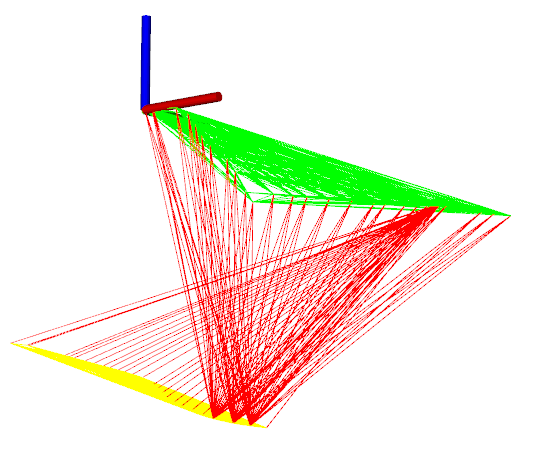
\includegraphics[scale=0.21]{gfx/covgraph_minHits_5_skip_1}}
    \subcaptionbox{10 \gls{KF} skipped after a \gls{KF} match}{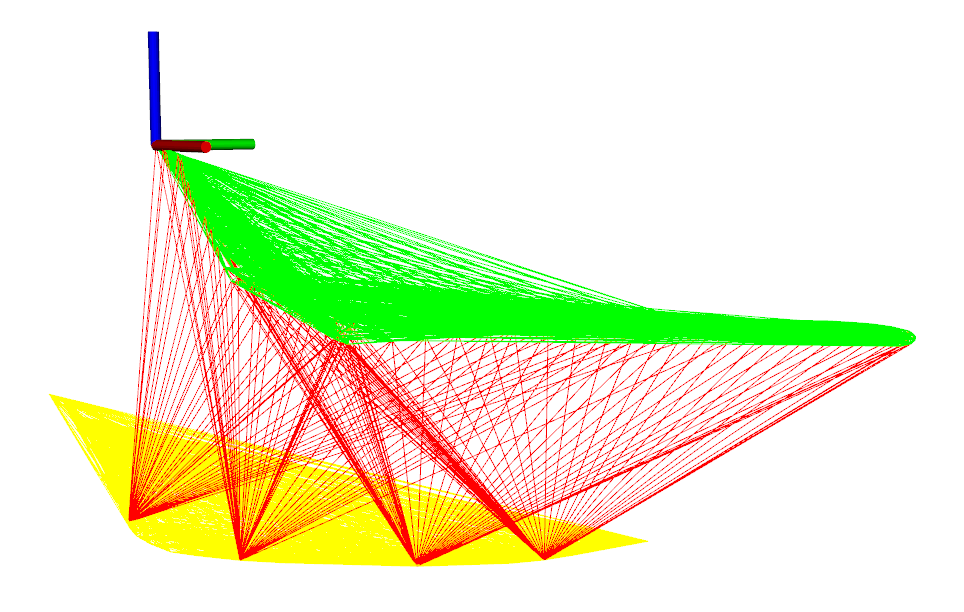
\includegraphics[scale=0.17]{gfx/covgraph_minHits_5_skip_10}}
  \end{figure}
}

\frame{
  \frametitle{Map merging - Results - Reduction of drift}
  \begin{figure}[H]
    \centering
    \subcaptionbox{original approach}{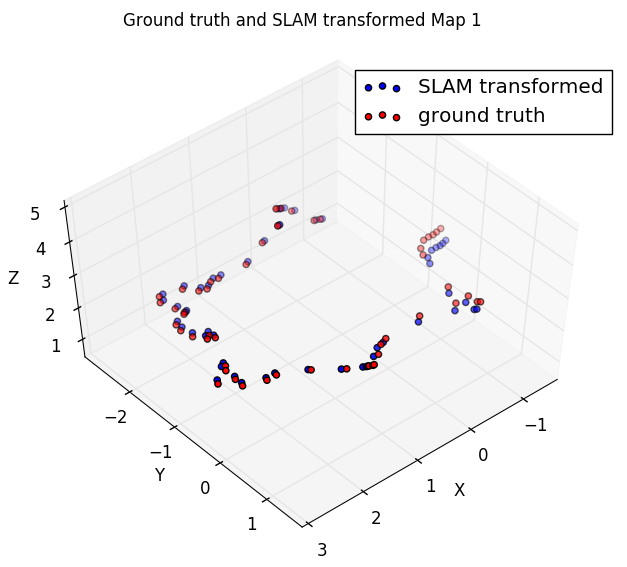
\includegraphics[scale=0.225]{gfx/m1_skf0_cut}}
    \subcaptionbox{new approach}{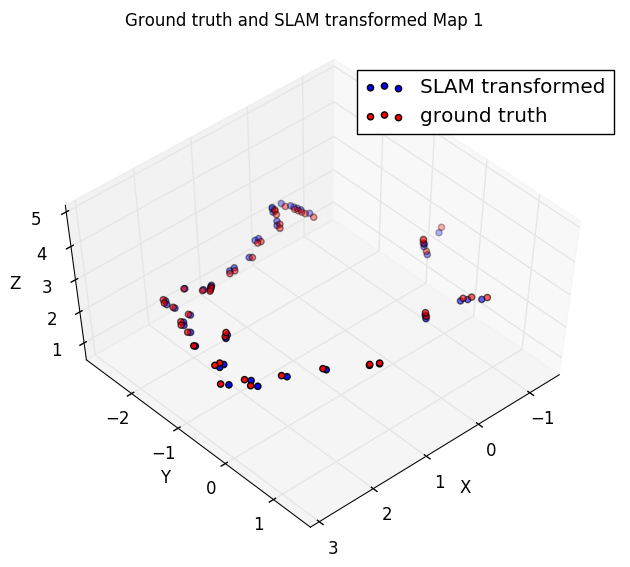
\includegraphics[scale=0.225]{gfx/m10_skf10_cut}}
  \end{figure}

}

\section{Culling}
\frame{\tableofcontents[currentsection]}

\frame{
  \frametitle{Culling - Remove redundant \gls{KF}}
  \begin{itemize}
    \visible<1-4>{
    \item Remove redundant \gls{KF} after $n$ \gls{KF} matches were found
    }
    \visible<2-4>{
    \item{Performs culling for every \gls{KF} match separately
    }
      \begin{itemize}
        \visible<3-4>{
        \item Check \gls{KF}s which are directly connected to one of the \gls{KF}s in the co-visibility graph
        }
        \visible<4>{
        \item If x\% of the observations of a \gls{KF} are also observed in another \gls{KF}, this \gls{KF} will be deleted.
        }
      \end{itemize}
    }

  \end{itemize}

  \visible<3-4>{
  \begin{center}
    \begin{tikzpicture}[auto]
      \node[entity] (key frame match) {kf match}
        [grow=down,sibling distance=4.5cm]
        child {node[entity] (child 1) {kf, map 1}
          [grow=down,sibling distance=1.2cm]
          child {node[entity,minimum size=1cm] {kf 1}}
          child {node[entity,minimum size=1cm] {kf 2}}
          child {node[entity,minimum size=1cm] {kf $k$}}}
        child {node[entity] {kf, map 2}
          [grow=down,sibling distance=1.2cm]
          child {node[entity,minimum size=1cm] {kf 1}}
          child {node[entity,minimum size=1cm] {kf 2}}
          child {node[entity,minimum size=1cm] {kf $l$}}};
    \end{tikzpicture}
  \end{center}
  }
}

\subsection{Results}
\frame{
  \frametitle{Culling - Results}
  PGO := pose graph optimization\\
  GBA := global bundle adjustment\\

  \begin{table}[ht!]
  \begin{center}
  \begin{tabular}{c|c|c|c|c}
    Culling &  \# matches & \# \gls{KF}s skipped & PGO [ms] & GBA [ms] \\ 
    \hline 
    No & 1 & 0 &142.25 & 163.89 \\
    Yes & 1 & 0 & 42.01 & 72.33 \\
    No & 10 & 10 & 532.28 & 3659.48 \\
    Yes & 10 & 10 & 178.83 & 1098.37 \\
    %\hline 
  \end{tabular}
  \end{center}
  \caption{Time measurements of PGO and GBA without and with culling.}
  \label{tab:results_time}
  \end{table}
}

\frame{
  \frametitle{Culling - Results}
  \begin{table}[ht!]
  \begin{center}
  \begin{tabular}{c|c|c|c}
    Culling &  \# matches & \# \gls{KF}s skipped & \textit{rmse} [m] \\ 
    \hline 
    No & 1 & 0 & 0.1310 \\
    Yes & 1 & 0 & 0.2187 \\
    No & 10 & 10 & 0.0961 \\
    Yes & 10 & 10 & 0.0965 \\
    %\hline 
  \end{tabular}
  \end{center}
  \caption{\textit{rmse} without and with culling.}
  \label{tab:results_rmse}
  \end{table}
}

\section{Use dog leg optimizer for GBA}
\frame{\tableofcontents[currentsection]}

\frame{
  \frametitle{Use dog leg optimizer for GBA}
  As proposed in \cite{Lourakis2005}
}

\section{Results}
\frame{\tableofcontents[currentsection]}

\begin{frame}
	\frametitle{Results}
	\begin{itemize}
	\visible<1-6>{
	\item The measurements of a motion detection system (VICON) serve as ground truth
	}
	\visible<2-6>{
	\item For comparison the $\textit{rmse}$ and the $\textit{rmse}_{xy}$ of the EKF and of the UWB system were calculated and compared
	}
	\visible<3-6>{
	\item The accuracy of the EKF is at least doubled compared to the UWB system
	}
	\visible<4-6>{
	\item For the cases, where the visual tracker found the object
	}
	\visible<5-6>{
	\item Inaccuracies in the system are possible
	}
	\end{itemize}
	%\tiny
	%\begin{table}
%		\begin{center}
%			\begin{tabular}{c|c|c|c|c}
%				Experiment number & $\textit{rmse}$ of UWB & $\textit{rmse}$ of EKF & $\textit{rmse}_{xy}$ of UWB & $\textit{rmse}_{xy}$ of EKF\\ 
%				\hline 
%				1 & 0.0667 & 0.0350 & 0.0621 & 0.0270 \\
%				2 & 0.0771 & 0.0364 & 0.0734 & 0.0260 \\
%				3 & 0.1304 & 0.0379 & 0.1275 & 0.0312 \\
%				4 & 0.1169 & 0.0344 & 0.1126 & 0.0265 \\
%				5* & 0.1273 & 0.1195 & 0.1159 & 0.1055
				%\hline 
%			\end{tabular}
%		\end{center}
%	\end{table}
%	\normalsize
	\vspace{1cm}
	\visible<6>{
	See demo video!
	}
\end{frame}

\section{Conclusion}
\frame{\tableofcontents[currentsection]}

\subsection{Conclusion}
\frame { \frametitle{Conclusion/Limitation}
	Conclusion:
	\begin{itemize}
	\pause
	\item The proposed method of fusing UWB and visual tracker impoved the accuracy
	\pause
	\item The implemented re-detection mechanism performs well
	\end{itemize}

	\pause
	Limitation:
	\begin{itemize}
	\pause
	\item The EKF does not consists of an outlier-detection
	\pause
	\item Parameter tuning required for the re-detection mechanism
	\end{itemize}
}

\subsection{Outlook}
\frame { \frametitle{Outlook}
	Outlook:
	\begin{itemize}
	\pause
	\item Profiling/C++ implementation for usage with higher frequency
	\pause
	\item More sophisticated re-detection
	\pause
	\item Calibration of the UWB system with the help of ArUco
	\pause
	\item Automatic target detection/learning
	\pause
	\item Multi target tracking
	\end{itemize}
}

\frame { \frametitle{Questions}
	\section{Questions}
	\begin{center}
	
\includegraphics[height=0.75\textheight]{gfx/q&a.jpg}
	\end{center}
}

\frame{ \frametitle{References}
	\section{References}
	\bibliography{references}
}

\end{document}
